\section{Gruppen und Symmetrie}
\label{gruppentheorie}

\begin{bemerkung}
Wir möchten Gruppentheorie zunächst motivieren: Man betrachte einen Tetraeder. Um dessen Symmetrien zu erfassen, könnten wir z.B. schauen, welche Bewegungen diesen in sich selbst überführen. Es gibt vier Rotationsachsen, die eine Ecke und eine Fläche durchdringen und bei Rotation um $120^\circ$ den Tetraeder in sich selbst überführen. Weiterhin gibt es drei $180^\circ$-Rotationsachsen mittig durch gegenüberliegende Kanten. Auch die Identität lässt den Tetraeder unverändert. Also gibt es $1+4 \cdot 2 + 3 = 12$ Symmetrien. Gruppen bieten eine Möglichkeit, solche Symmetrien und deren Verkettungen zu erfassen und zu untersuchen.
\end{bemerkung}

\subsection{Grundbegriffe}
\label{subsec:grundbegriffe}

\begin{definition}{Gruppe}{gruppe}
Eine \textbf{Gruppe} ist ein Paar $(G, \circ)$, bestehend aus einer Menge\footnote{im ZFC-Axiomensystem} $G$ und einer Abbildung
\begin{align}
\circ: G \times G &\to G\\
(g,h) &\mapsto g \circ h
\end{align} 
mit folgenden Eigenschaften:
\begin{enumerate}[({G}1)]
\item Für alle $g_1,g_2,g_3 \in G$ gilt das Assoziativgesetz: $(g_1 \circ g_2) \circ g_3 = g_1 \circ (g_2 \circ g_3)$.
\item Es gibt ein Element $e \in G$, sodass gilt:
\begin{enumerate}[({2}a)]
\item Für jedes $g \in G$ gilt $e \circ g = g$.
\item Für jedes $g \in G$ existiert ein $g' \in G$ mit $g' \circ g = e$.
\end{enumerate}
\end{enumerate}
Die Abbildung $\circ$ heißt \textbf{Verknüpfung}, ein Element $e \in G$ mit den Eigenschaften aus (2G) heißt \textbf{neutrales Element}, und ein Element $g' \in G$ zu gegebenem $g \in G$ mit Eigenschaft (2b) heißt \textbf{Inverses} von $g$.
\end{definition}

\begin{übung}
Sei $(G, \circ)$ eine Gruppe. Dann gelte:
\begin{enumerate}
\item Das neutrale Element $e \in G$ ist eindeutig bestimmt, außerdem gelte $ \forall g \in G : g \circ e = g$.
\item Zu gegebenem $g \in G$ ist das Inverse $g' \in G$ eindeutig bestimmt und erfüllt zudem $g \circ g' = e$.
\item Für $n \geq 3$ hängt das Produkt von Gruppenelementen $g_1, g_2, \dots, g_n$ nicht von der Klammerung ab.
\end{enumerate}
\end{übung}

\begin{lösung}
Zuerst zeigen wir Kommutativität des Inversen. Sei $g \in G$, dann gilt:
\begin{align}
g \circ g^{-1} &= (e \circ g) \circ g^{-1} = \left( \left( \left( g^{-1}\right)^{-1} \circ g^{-1} \right) \circ g \right) \circ g^{-1} = \left(  \left( g^{-1}\right)^{-1} \circ \left( g^{-1} \circ g \right)\right) \circ g^{-1}\\ 
&= \left( g^{-1}\right)^{-1} \circ \left( e  \circ g^{-1} \right) = \left( g^{-1}\right)^{-1} \circ g^{-1} = e = g^{-1} \circ g,
\end{align}
also stimmen Links- und Rechtsinverses in Gruppen überein.
Die Kommutativität des neutralen Elements folgt damit direkt aus:
\begin{equation}
g \circ e = g \circ (g^{-1} \circ g) = (g \circ g^{-1}) \circ g = (g^{-1} \circ g) \circ g = e \circ g,
\end{equation}
womit auch Links-Einselement und Rechts-Einselement übereinstimmen.
Für die Eindeutigkeit des Inversen seien $g^{-1}, g'^{-1} \in G$ zwei Inverse von $g \in G$. Dann gilt:
\begin{equation}
g^{-1} = g^{-1} \circ e = g^{-1} \circ (g'^{-1} \circ g) = g^{-1} \circ (g \circ g'^{-1}) = (g^{-1} \circ g) \circ g'^{-1} = e \circ g'^{-1} = g'^{-1}.
\end{equation}
Weiterhin seien $e,e' \in G$ zwei Einselemente. Da $e = e \circ e' = e' \circ e = e$ gilt, ist das neutrale Element eindeutig. \qed
\end{lösung}

\begin{beispiele}
Wir geben einige Beispiele für Gruppen:
\begin{enumerate}
\item Die Gruppe $(\Z, +)$ der ganzen Zahlen $\Z$ mit der Addition $+$.
\item Für einen Körper $\K$ existiert die additive Gruppe $(\K, +)$ und die multiplikative Gruppe $(\K \exc \{0\}, \cdot)$.
\item Für jede Menge $M$ existiert die \textbf{symmetrische Gruppe} $(\mathfrak{S}_M, \circ)$, wobei $\mathfrak{S}_M$ die Menge der bijektiven Selbstabbildungen von $M$ und $\circ$ die Komposition ist. Für $n \geq 1$ vereinbaren wir $\mathfrak{S}_n := \mathfrak{S}_{\{1,2,\dots,n\}}$. Wir vereinbaren als Konvention die \textbf{Zykelschreibweise}. In $\mathfrak{S}_3$ beispielsweise ist ein Zykel
\begin{align}
\sigma: \{1,2,3\} &\to \{1,2,3\}\\
1 &\mapsto 2 \\
2 &\mapsto 1 \\
3 &\mapsto 3,
\end{align}
auch darstellbar als
\begin{equation}
\mat{1,2,3}{2,1,3}
\end{equation}
oder einfacher als $(12)$.
\item Für $n \geq 1$ und einen Körper $\K$ ist die \textbf{allgemeine lineare Gruppe} $(\text{GL}(n,\K), \circ)$ definiert, wobei 
\begin{equation}
\text{GL}(n, \K) := \left\{ A \in \K^{n\times n} \, | \, \det A \neq 0 \right\}
\end{equation}
die Menge der invertierbaren $n \times n$-Matrizen mit Einträgen in $\K$ ist. Typische Beispiele für Körper sind $\K = \Q, \R, \C, \F_q$ mit $q = p^n$, $p$ prim.\\
ÜA: $| \text{GL}(n, \F_q)| = ?$.
\end{enumerate}
\end{beispiele}
\begin{bemerkung}
Um den alltäglichen Gebrauch von Gruppen zu vereinfachen, machen wir folgende Vereinbarungen:
\begin{enumerate}
\item Wir bezeichnen $(G, \circ)$ üblicherweise einfach mit $G$ und lassen $\circ$ implizit.
\item Für $g,h \in G$ schreiben wir $gh = g \circ h$, für $e \in G$ schreiben wir $1$ und für $g'$ schlicht $g^{-1}$.
\item Gilt $g \circ h = h \circ g$ für alle $g,h \in G$, so heißt $G$ \textbf{abelsch}. In diesem Fall wird die Verknüpfung oft mit $+$, das neutrale Element mit $0$ und das inverse Element mit $-g$ bezeichnet.
\item Gemäß obiger ÜA zur Klammerung schreiben wir einfach $g_1 g_2 \cdots g_n \in G$ ohne Klammerung.
\end{enumerate}
\end{bemerkung}
\begin{definition}{Ordnung}{ordnung}
Für eine Gruppe $G$ bezeichnen wir die Kardinalität \begin{equation}
|G| \in \N \cup \{+\infty \}
\end{equation}
als \textbf{Ordnung} von $G$.
\end{definition}

\subsection{Untergruppen}
\label{subsec:untergruppen}
\begin{definition}{Untergruppe}{untergruppe}
Sei $(G, \circ)$ eine Gruppe. Eine Teilmenge $H \sub G$ heißt \textbf{Untergruppe}, falls gilt:
\begin{enumerate}[({U}1)]
\item $H \neq \emptyset$
\item Abgeschlossenheit: Für alle $a, b \in H$ gilt $ab^{-1} \in H$.
\end{enumerate}
Wir verwenden dann die Notation $H \leq G$, um Untergruppen zu kennzeichnen.
\end{definition}

\begin{bemerkung} Übungsaufgabe:
Sei $G$ eine Gruppe und $H \leq G$ eine Untergruppe. Dann gilt:
\begin{enumerate}
\item Aus Eigenschaft 1:Da $H \neq \emptyset$, existiert ein $a \in H$.
\item Aus Eigenschaft 2: $a \cdot a^{-1} = e \in H$.
\item Aus Eigenschaft 2: Für jedes $a \in H$ gilt $a^{-1} = e \cdot a^{-1} \in H$.
\item Aus Eigenschaft 2: Für jedes $a,b \in H$ gilt $ab = a \cdot (b^{-1})^{-1} \in H$.
\end{enumerate}
Also: $H \sub G$ ist eine Untergruppe genau dann, wenn folgende alternativen Eigenschaften gelten:
\begin{enumerate}[1.{$^\ast $}]
\item $e_G \in H$
\item Für alle $a,b \in H$ muss $a \cdot b \in H$ gelten.
\item Für alle $a \in H$ ist $a^{-1} \in H$.
\end{enumerate}
Die andere Richtung der Äquivalenz ist trivial. Daraus folgt auch, dass $(H, \circ|_{H \times H})$ mit der auf $H$ eingeschränkten Verknüpfung $\circ|_{H \times H}$ eine Gruppe ist. 
\end{bemerkung}
\begin{beispiele}
Einige Beispiele für Untergruppen sind:
\begin{enumerate}
\item $(G, \circ) = (\R, +)$ hat $(\Z, +)$ als Untergruppe mit $\Z \sub \R$.
\item Sei $n \geq 1$ und $\K$ ein Körper. Die \textbf{spezielle lineare Gruppe}
\begin{equation}
\text{SL} (n, \K) := \left\{ A \in \text{GL}(n, \K) \, | \, \det A = 1\right\} \leq \text{GL}(n, \K)
\end{equation}
ist eine Untergruppe von $\text{GL}(n,\K)$.
\item Für $n \geq$ und einen Körper $\K$ ist die \textbf{orthogonale Gruppe}
\begin{equation}
\text{O}(n, \K) := \left\{ A \in \text{GL}(n, \K) \, | \, A^TA = I_n \right\} \leq \text{GL}(n, \K)
\end{equation}
definiert, die auch eine Untergruppe von $\text{GL}(n, \K)$ ist.
\item Seien $H_1, H_2 \leq G$ Untergruppen. Dann ist $H_1 \cap H_2 \leq G$ auch eine Untergruppe. So kann z.B. die \textbf{spezielle orthogonale Gruppe}
\begin{equation}
\text{SO}(n, \K) := \text{O}(n, \K) \cap \text{SL}(n, \K)
\end{equation}
als Untergruppe von $\text{GL}(n, \K)$ konstruiert werden.
\item Etwas allgemeiner: Für jede Familie $\{H_i\}_{i\in I}$ von Untergruppen $H_i \leq G$ gilt, dass
\begin{equation}
\bigcap_{i \in I} H_i \leq G
\end{equation}
wieder eine Untergruppe ist.
\end{enumerate}
\end{beispiele}
\begin{definition}{Erzeugte Untergruppe}{}
Sei $G$ eine Gruppe und $M \sub G$ eine beliebige Teilmenge. Dann heißt die \textbf{Untergruppe}
\begin{equation}
\langle M \rangle := \bigcup_{M \sub H \leq G} H \leq G
\end{equation}
die \textbf{von} $M$ \textbf{erzeugte Untergruppe} von $G$. Falls $M = \{g\} \leq G$ eine einelementige Menge ist, schreiben wir \begin{equation}
\langle g \rangle := \langle \{g\} \rangle \leq G.
\end{equation}
\end{definition}
\begin{definition}{Ordnung eines Elements}{ordnungelement}
Sei $G$ eine Gruppe und $g \in G$ ein Element. Dann heißt die Kardinalität 
\begin{equation}
\text{ord}(g) := | \langle g \rangle | \in \N \cup \{\infty \}
\end{equation}
die \textbf{Ordnung von} $g$.
\end{definition}
\begin{satz}{Charakterisierung von einelementigen Untergruppen}{charakterisierungeinelementig}
Sei $G$ eine Gruppe und $g \in G$ ein Element.
\begin{enumerate}
\item Falls $\ord (g) < \infty$, dann gilt \begin{equation}
\ord (g) = \min \{k \geq 1 | g^k= 1\}
\end{equation}
und \begin{equation}
\langle g \rangle = \{1, g, g^2, \dots, g^{n-1} \},
\end{equation}
wobei $n := \ord (g)$.
\item Falls $\ord (g) = \infty$, dann gilt
\begin{equation}
\langle g \rangle = \{g^i | i \in \Z \} = \{ \dots, g^{-2}, g^{-1}, 1, g^1, g^2, \dots \},
\end{equation}
wobei die Potenzen $g^i$, $i \in \Z$ paarweise verschiedene Elemente in $G$ sind.
\end{enumerate}
\end{satz}
\begin{beweis}
Zunächst gilt für beliebiges $g \in G$ das Folgende:
\begin{equation}
\langle g \rangle = \{ \dots,g^{-2},g^{-1},1, g, g^2, \dots \} = \{g^i | i \in \Z\},
\end{equation}
wobei die Potenzen im Allgemeinen nicht notwendigerweise paarweise verschieden sind.
Dies folgt, da, damit $\langle g \rangle$ eine Untergruppe sein kann, zunächst das neutrale Element $1 = g^0$ und $g$ selbst enthalten sein muss. Dann muss aber auch die Selbstverknüpfung und das Inverse (sowie dessen Selbstverknüpfungen) enthalten sein.
\begin{enumerate}
\item Sei $\ord (g) < \infty$. Dann gibt es insbesondere $i,j \in \Z$ mit $i \neq j$ und $g^i = g^j$. O.B.d.A. sei $i > j$. Dann ist also $k = i-j \geq 1$ eine natürliche Zahl, für die gilt: $g^k = 1$. Nach dem Wohlordnungssatz existiert eine \textit{kleinste} natürliche Zahl $n \geq 1$, für die gilt: $g^n =1$. Sei nun $m \in \Z$. Dann gibt es eindeutig bestimmte Zahlen $a \in \Z$ und $0 \leq r < n$, sodass \begin{equation}
m = an +r.
\end{equation}
Damit folgt
\begin{equation}
g^m = g^{an+r} = (\underbrace{g^n}_{=1})^a \cdot g^r = g^r.
\end{equation}
Dies impliziert $\langle g \rangle = \{1,g,g^2,\dots, g^{n-1}\}$, da $r$ der Rest ist, der bei der Division von $n$ durch $m$ bleibt. Die möglichen Reste für gegebenes $n$ legen also die Elemente von $G$ fest.\\
Wir müssen noch zeigen, dass $1, g, \dots, g^{n-1}$ paarweise verschieden sind. Dies folgt allerdings direkt aus der Tatsache, dass $n$ minimal ist.
\item Das obige Argument zeigt per Kontraposition auch 2., denn wenn die Potenzen $g^i$, $i \in \Z$ nicht paarweise verschieden sind, dann zeigt obiges Argument, dass $\langle g \rangle = \{1,g,\dots, g^{n-1}\}$ für $n \in \N$, was ein Widerspruch zur Annahme $\ord (g) = \infty$ ist.
\end{enumerate}
\end{beweis}
\begin{definition}{zyklische Gruppe}{zyklisch}
Sei $G$ eine Gruppe. Existiert ein $g\in G$, sodass sich jedes $h \in G$ als $g^n = h$ für ein $n \in \Z$ schreiben lässt, heißt $G$ \textbf{zyklisch der Ordnung} $\ord (g)$. Das Element $g$ heißt \textbf{Erzeuger von} $G$.
\end{definition}
\subsection{Homomorphismen}
\label{subsec:homomorphismen}
\begin{definition}{Homomorphismus}{homomorphismus}
Seien $G$ und $G'$ Gruppen. Eine Abbildung 
\begin{equation}
\phi: G \to G'
\end{equation}
heißt \textbf{(Gruppen-)Homomorphismus}, falls gilt:
\begin{enumerate}[({H}1)]
\item Für alle $g,h \in G$ gilt 
\begin{equation}
\phi(gh) = \phi(g) \cdot \phi(h).
\end{equation}
Die Menge der Homomorphismen von $G$ nach $G'$ wird mit $\Hom (G, G')$ bezeichnet.
\end{enumerate}
\end{definition}
\begin{bemerkung}
Jeder Homomorphismus erfüllt außerdem folgende Eigenschaften, die aus Definition \ref{homomorphismus} folgen:
\begin{enumerate}[({H}1)]
\setcounter{enumi}{1}
\item $\phi (1_G) = 1_{G'}$
\item Für alle $g \in G$ gilt $\phi (g^{-1}) = \phi (g)^{-1}$.
\end{enumerate}
Das sieht man schnell, da $\phi(1) = \phi(1g) = \phi(1) \phi(g)$ gilt, also $\phi(1) = 1'$ sein muss. Weiterhin gilt $1' = \phi(1) = \phi(gg^{-1}) = \phi(g) \phi(g^{-1})$, Linksmultiplikation mit $\phi^{-1}(g)$ liefert (H3).
\end{bemerkung}
\begin{beispiele}
\begin{enumerate}
\item Die \textbf{Einbettung} $\phi: H \hookrightarrow G$ einer Untergruppe $H \leq G$ ist ein Homomorphismus.
\item Die \textbf{Determinantenabbildung}
\begin{equation}
\det: \text{GL} (n, \K) \to (\K \exc \{0\}, \cdot)
\end{equation}
ist ein Homomorphismus.
\item Für $n \geq 1$ und einen Körper $\K$ ist die Permutationsabbildung
\begin{align}
P: \mathfrak{S}_n &\to \text{GL}(n, \K) \\
\sigma &\mapsto P_\sigma,
\end{align}
mit der \textbf{Permutation}
\begin{equation}
(P_\sigma)_{ij} := \begin{cases} 1 \, \text{falls} \, i = \sigma(j)\\0 \, \text{sonst} \end{cases}
\end{equation}
ein Homomorphismus. \textit{Der Beweis sei dem Leser überlassen.}
Für $\sigma = (123) \in \mathfrak{S}_3$ gilt z.B. 
\begin{equation}
P_\sigma = \mat{0,0,1}{1,0,0}{0,1,0}.
\end{equation}
\item Sei $G$ eine Gruppe und $g \in G$. Dann ist 
\begin{align}
\gamma_g: G &\to G \\
h &\mapsto ghg^{-1}
\end{align}
ein Homomorphismus, genannt \textbf{Konjugation mit} $g$.
\item Sei $G$ eine Gruppe und $g \in G$. Dann ist 
\begin{align}
\Z &\to G \\
i &\mapsto g^i
\end{align}
ein Homomorphismus von $(\Z, +)$ nach $(G, \circ)$.
\end{enumerate}
\end{beispiele}
\begin{definition}{Isomorphismus}{isomorphismus}
Sei $\phi$ ein Gruppenhomomorphismus, der zusätzlich bijektiv ist. Dann heißt $\phi$ \textbf{Isomorphismus}. Zwei Gruppen $G$ und $G'$ heißen \textbf{isomorph}, in Zeichen $G \cong G'$, falls es einen Isomorphismus zwischen ihnen gibt.
\end{definition}
\begin{bemerkung}
Anschaulich bedeutet das, dass zwei isomorphe Gruppen identisch bis auf Umbenennung ihrer Elemente sind.
\end{bemerkung}
\begin{beispiele}
\begin{enumerate}
\item Die Permutationsabbildung $P$ induziert einen Isomorphismus
\begin{align}
P: \mathfrak{S}_n &\to P(n, \K)\\
\sigma &\mapsto P_\sigma
\end{align}
zwischen der symmetrischen Gruppe und der Untergruppe der Permuationsmatrizen. Letztere sind Matrizen, die in jeder Zeile und Spalte \textit{genau eine} $1$ und sonst $0$ haben. \textit{Der Beweis sei dem Leser überlassen.}
\item Die \textbf{Exponentialfunktion}
\begin{equation}
\exp: (\R, +) \to (\R_{> 0}, \cdot)
\end{equation}
und ihre Umkehrfunktion, gegeben durch den \textbf{Logarithmus}
\begin{equation}
\ln: (\R_{>0}, \cdot) \to (\R, +),
\end{equation}
bilden einen Isomorphismus, also gilt $(\R, +) \cong (\R_{>0}, \cdot)$.
\end{enumerate}
\end{beispiele}
\begin{definition}{Bild und Kern}{bildkern}
Sei $\phi: G \to G'$ ein Gruppenhomomorphismus. Dann heißt die Teilmenge
\begin{equation}
\im (\phi) := \{g' \in G' | \exists g \in G: \phi(g) = g'\} \leq G',
\end{equation}
das \textbf{Bild von} $\phi$ und die Teilmenge
\begin{equation}
\ker (\phi) := \{g \in G|\phi(g) = 1_{G'} \} \leq G,
\end{equation}
der \textbf{Kern von} $\phi$.
\end{definition}
\begin{satz}{Bild und Kern sind Untergruppen}{bildkernuntergruppe}
Sei $\phi: G \to G'$ ein Gruppenhomomorphismus. Dann sind $\im (\phi) \leq G'$ und $\ker (\phi) \leq G$ Untergruppen der jeweiligen Gruppen $G$ und $G'$.
\end{satz}
\begin{beweis}
Nachrechnen mittels (H1), (H2) und (H3), exemplarisch für den Kern gezeigt:
\begin{enumerate}
\item (U1) ist erfüllt, da $1_G \in \ker (\phi)$ wegen (H2) gilt.
\item (U2) kann nachgerechnet werden. Seien dafür $g,h \in \ker (\phi)$:
\begin{equation}
\phi(gh^{-1}) =^{\text{(H1)}} \phi(g) \cdot \phi(h^{-1}) =^{\text{(H3)}} \phi(g) \cdot \phi(h)^{-1} = 1_{G'},
\end{equation}
also $gh^{-1} \in \ker (\phi)$.
\end{enumerate}
\end{beweis}
\begin{satz}{}{}
Für einen Homomorphismus $\phi: G \to G'$ sind folgende Aussagen äquivalent:
\begin{enumerate}[(i)]
\item $\phi$ ist injektiv.
\item $\ker (\phi) = \{1\}$
\end{enumerate}
\end{satz}
\begin{beweis}
(i) $\implies$ (ii) ist offensichtlich. Wir zeigen noch (ii) $\implies$ (i):
Sei also $\ker (\phi) = \{1\}$ und $g,h \in G$ mit $\phi(g) = \phi(h)$. Dann gilt $\phi(gh^{-1})=\phi(g)\phi(h)^{-1} =1$, also ist $gh^{-1} \in \ker (\phi) = \{1\}$ und damit $g = h$.
\end{beweis}
\begin{definition}{Links- und Rechtsnebenklassen}{linksrechtsnebenklasse}
Sei $G$ eine Gruppe und $H \leq G$ eine Untergruppen. Dann ist die \textbf{Linksnebenklasse von} $H$ \textbf{bezüglich} $g \in G$ als 
\begin{equation}
gH := \{gh \, | \, h \in H\}
\end{equation}
und die \textbf{Rechtsnebenklasse von} $H$ \textbf{bezüglich} $g \in G$ als 
\begin{equation}
Hg := \{hg \, | \, h \in H \}
\end{equation}
definiert.
\end{definition}
\begin{satz}{Nebenklassen sind Äquivalenzklassen}{nebenklassenäquivalenzrel}
Sei $G$ eine Gruppe und $H \leq G$ eine Untergruppe. Dann gilt:
\begin{enumerate}
\item Die Linksnebenklassen sind die Äquivalenzklassen bezüglich der Äquivalenzrelation
\begin{equation}
a \sim_L b :\iff b^{-1}a \in H
\end{equation}
auf $G$.
\item Die Rechtsnebenklassen sind die Äquivalenzklassen bezüglich der analogen Äquivalenzrelation
\begin{equation}
a \sim_R b : \iff ab^{-1} \in H.
\end{equation}
\end{enumerate}
\end{satz}
\begin{übung}
Beweis des Satzes.
\end{übung}
\begin{lösung}
Zunächst ist zu zeigen, dass tatsächlich eine Äquivalenzrelation definiert wird.\\
\begin{enumerate}[(a)]
\item Reflexivität: Sei $a \in G$. Dann gilt $a^{-1}a = 1 \in H$, also ist $a \sim_L a$.
\item Symmetrie: Seien $a,b \in G$ mit $a \sim_L b$. Dann gilt $a^{-1} b = h$ für ein $h \in H$. Daraus folgt:
\begin{equation}
a = bh \iff ah^{-1} =b \iff a^{-1}b = h^{-1} \in H,
\end{equation}
also ist auch $b \sim_L a$, da $H$ abgeschlossen unter Inversenbildung ist.
\item Transitivität: Seien $a,b,c \in G$ mit $a \sim_L b$ und $b \sim_L c$. Dann gilt $b^{-1}a = h \in H$ und $c^{-1} b = h' \in H$. Also folgt $H \ni h'h = c^{-1}bb^{-1}a = c^{-1} a$ und damit die Behauptung.
\end{enumerate}
Ist nun $g \in G$ und $h \in H$, so besteht die Äquivalenzklasse von $g$ unter $\sim_L$ aus allen Elementen der Form $ah$ mit $a \in G$, $h \in H$. Die Vereinigung aller Äquivalenzklassen muss also per Konstruktion ganz $gH$ sein. Der Beweis für $\sim_R$ ist dual dazu. \qed
\end{lösung}

Damit bezeichnen wir die Menge der Linksnebenklassen von $H$ mit $\quotient{G}{H} = \quotient{G}{\sim_L}$ und die der Rechtsnebenklassen mit $\invquotient{G}{H} = \quotient{G}{\sim_R}$.
\begin{definition}{Index}{index}
Die Kardinalität
\begin{equation}
(G : H) := \left| \quotient{G}{H} \right| \in \N \cup \{\infty\}
\end{equation}
heißt \textbf{Index von} $H$ \textbf{in} $G$.
\end{definition}
Man beachte, dass $\left| \quotient{H}{G} \right| = \left| \invquotient{H}{G} \right|$ gilt, da die Abbildung \textcolor{red}{Tafel nicht hochgeschoben...}.
\begin{theorem}{Satz von Lagrange}{satzvonlagrange}
Sei $G$ eine Gruppe und $H \leq G$ eine Untergruppe. Dann gilt 
\begin{equation}
|G| = (G : H) \cdot |H|.
\end{equation}
Ist $|G| < \infty$, so gilt insbesonders
\begin{equation}
(G : H) = \frac{|G|}{|H|} = \left| \quotient{G}{H} \right|.
\end{equation}
\end{theorem}
\begin{beweis}
Dies ist ein direktes Korollar von Satz \ref{nebenklassenäquivalenzrel}: Als Äquivalenzklassen bzgl. einer Äquivalenzrelation bilden die Linksklassen eine Partition von $G$, also 
\begin{equation}
G = \bigsqcup_{gH \in \quotient{G}{H}} gH.
\end{equation}
Es gilt zudem für alle $g \in G$, dass $|gH| = |H|$, da Linksmultiplikation mit $g$, definiert durch 
\begin{align}
G &\to G\\
x &\mapsto gx,
\end{align}
bijektiv ist, also eine Bijektion $H \to gH$ induziert. Insbesondere gilt für jedes $g \in G$, dass $\ord (g) \mid |G|$.
\end{beweis}
\begin{definition}{Normalteiler}{normalteiler}
Eine Untergruppe $N \leq G$ heißt \textbf{normal} oder \textbf{Normalteiler}, falls für alle $g \in G$ 
\begin{equation}
gN = Ng
\end{equation}
gilt. Wir schreiben dafür $N \trianglelefteq G$.
\end{definition}
\begin{bemerkung}
Eine Untergruppe $N \leq G$ ist normal genau dann, wenn für alle $g \in G$ und $n \in N$ gilt:
\begin{equation}
gng^{-1} \in N,
\end{equation}
also $N$ abgeschlossen unter Konjugation mit beliebigen Elementen aus $G$ ist.
\end{bemerkung}
\begin{satz}{}{}
Sei $\phi: G \to G'$ ein Gruppenhomomorphismus. Dann gilt $\ker (\phi) \trianglelefteq G$.
\end{satz}
\begin{beweis}
Sei $g \in G$ und $x \in \ker (\phi)$, also $\phi (x) = 1$. Dann gilt auch 
\begin{equation}
\phi (gxg^{-1}) = \phi(g)\underbrace{\phi(x)}_{=1}\phi(g^{-1}) = \phi(g)\phi(g)^{-1} = 1.
\end{equation}
\end{beweis}
\begin{beispiele}
Wir betrachteten einige Beispiele für Normalteiler:
\begin{enumerate}
\item Sei $n \geq 1$ und $\K$ ein Körper. Für 
\begin{equation}
\det: \text{GL}(n,\K) \to \K^\ast
\end{equation}
gilt
\begin{equation}
\ker (\det) = \text{SL}(n, \K) \trianglelefteq \text{GL}(n,\K).
\end{equation}
\item Betrachte für $n \geq 1$ die Komposition
\begin{center}
\begin{tikzcd}
    \mathfrak{S}_n \arrow[r,"P"] & P(n, \Q) \arrow[r, "\det"] & \{+1, -1\}.
\end{tikzcd}
\end{center}
Also ist 
\begin{equation}
A_n := \ker (\sgn) \trianglelefteq \mathfrak{S}_n
\end{equation}
normal. $A_n$ heißt \textbf{alternierende Gruppe}.
\end{enumerate}
\end{beispiele}
\begin{satz}{Gruppenstuktur auf Nebenklassen}{nebenklassengruppen}
Sei $G$ eine Gruppe und $N \trianglelefteq G$. Dann gilt:
\begin{enumerate}
\item Auf der Menge $\quotient{G}{N}$ von Nebenklassen von $N$ existiert eine Gruppenstruktur mit Verknüpfung
\begin{align}
\quotient{G}{N} \times \quotient{G}{N} &\to \quotient{G}{N} \\
(aN, bN) &\mapsto abN.
\end{align}
\item Die Quotientenabbildung
\begin{align}
\pi: G &\to \quotient{G}{N}\\
a &\mapsto aN
\end{align}
ist ein Gruppenhomomorphismus mit $\ker (\pi) = N$.
\end{enumerate}
\end{satz}
\begin{beweis}
\begin{enumerate}
\item Zunächst muss die Wohldefiniertheit der Verknüpfung bewiesen werden. Seien $\tila \in aN$ und $\tilb \in bN$ Vertreter der Nebenklassen $aN$ und $bN$ $(\iff \tila N = aN)$. Dann existieren $m,n \in N$ mit $\tila = am$ und $\tilb = bn$. Nun gilt
\begin{equation}
\tila \cdot \tilb = am \circ bn = ab \circ \underbrace{b^{-1} mb}_{N \trianglelefteq G \implies \in N} \circ n \in N,
\end{equation}
also ist der Ausdruck wohldefiniert.
\begin{enumerate}[({G}1)]
\item Seien $aN, bN, cN \in \quotient{G}{N}$. Dann gilt
\begin{equation}
(aN \cdot bN) \cdot cN =^{\text{(G1) für G}} (ab)cN = a(bc)N = aN(bN \cdot cN).
\end{equation}
\item Neutrales Element: $1 \cdot N = N$
\item Inverses Element: $(aN)^{-1} = a^{-1} N$
\end{enumerate}
\item Es gilt 
\begin{equation}
\pi (ab)  = (ab)N = (aN)(bN)=\pi(a)\pi(b)
\end{equation}
nach Definition von $\pi$, also ist $\pi$ ein Homomorphismus. Darüber hinaus gilt
\begin{equation}
a \in \ker (\pi) \iff \pi(a) = 1_{\quotient{G}{H}} = N \iff aN = N \iff a \in N,
\end{equation}
also gilt $\ker (\pi) = N$.
\end{enumerate}
\end{beweis}
\begin{theorem}{Isomorphiesätze}{isomorphiesaetze}
\begin{enumerate}
\item Isomorphiesatz: Sei $\phi: G \to G'$ ein Gruppenhomomorphismus. Dann induziert $\phi$ einen Isomorphismus
\begin{align}
\overline{\phi} : \quotient{G}{\ker (\phi)} &\to \im (\phi)\\
g \ker (\phi) &\mapsto \phi(g).
\end{align}
\item Isomorphiesatz: Sei $H \leq G$ eine Untergruppe und $N \lnormal G$ eine normale Untergruppe. Dann definiert $g(N \cap H) \to gN$ einen Isomorphismus 
\begin{equation}
\quotient{H}{(N\cap H)} \to \quotient{NH}{N}.
\end{equation}
\item Seien $M, N \lnormal G$ und $M \leq N$. Dann ist $\quotient{N}{M} \lnormal \quotient{G}{M}$ und es existiert ein Isomorphismus
\begin{equation}
\quotient{(\quotient{G}{M})}{(\quotient{N}{M})} \to \quotient{G}{N}.
\end{equation}
\end{enumerate}
\end{theorem}
\begin{beweis}
Zunächst ist Wohldefiniertheit zu zeigen. Für $\tilg \in gN$, also $\tilg = gn$ für $n \in \ker (\phi)$, gilt:
\begin{equation}
\phi( \tilg) = \phi(gn) = \phi(g)\underbrace{\phi(n)}_{=1} = \phi(g),
\end{equation}
also ist die Abbildung wohldefiniert.\\
Die Surjektivität von $\overline{\phi}$ ist trivial. Wir wissen, dass $\overline{\phi}$ genau dann injektiv ist, wenn $\ker (\overline{\phi}) = \{1_{\quotient{G}{\ker (\phi) }}\} = \ker (\phi)$. Wir rechnen nach:
\begin{equation}
g \ker (\phi) \in \ker (\overline{\phi}) \iff \phi(g) = 1_{G'} \iff g \in \ker (\phi) \iff g \ker (\phi) = \ker (\phi)
\end{equation}
\end{beweis}
\begin{beispiel}
Wir können die Vorzeichenfunktion 
\begin{equation}
\sgn: \mathfrak{S}_n \to \{\pm 1\}
\end{equation}
betrachten, dann ist $\ker{\sgn} = A_n \trianglelefteq \Sf_n$, also erhalten wir einen Isomorphismus 
\begin{equation}
\quotient{\Sf_n}{A_n} \to \{ \pm 1\}.
\end{equation}
Insbesondere gilt $\Sf_n : A_n = 2$.
\end{beispiel}
\begin{korollar}{Korollar aus Satz \ref{isomorphiesaetze}}{korollarhomosatz}
Sei $\phi: G \to G'$ ein Gruppenhomomorphismus. Dann lässt sich $\phi$ schreiben als
\begin{equation}
\phi = \iota \circ \overline{\phi} \circ \pi,
\end{equation}
wobei:
\begin{enumerate}
\item $\pi:G \to \quotient{G}{\ker (\phi)}$ der surjektive Quotientenkern ist.
\item $\overline{\phi}: \quotient{G}{\ker (\phi)} \to \im (\phi)$ der Isomorphismus aus \ref{homomorphiesatz} ist.
\item $\iota: \im (\phi) \hookrightarrow G'$ die injektive Einbettung von $\im (\phi) \leq G'$ ist.
\end{enumerate}
Das ist äquivalent dazu, dass folgendes Diagramm kommutiert:
\begin{center}
\begin{tikzcd}
    G \arrow[r,"\phi"] \arrow[d, twoheadrightarrow, "\pi"] & G' \\
    \quotient{G}{\ker (\phi)} \arrow[r, "\cong", "\overline{\phi}"'] & \im (\phi) \arrow[u, hook, "\iota"]
\end{tikzcd}
\end{center}
Ausgedrückt in Elementen:
\begin{center}
\begin{tikzcd}
    g \arrow[r, mapsto] \arrow[d, mapsto] & \phi(g) \\
    g \ker (\phi) \arrow[r, mapsto] & \phi (g) \arrow[u, mapsto]
\end{tikzcd}
\end{center}
\end{korollar}
\begin{beispiele}
\begin{enumerate}
\item Für $n \geq 1$ und einen Körper $\K$ induziert der Homomorphismus
\begin{equation}
\det: \text{GL}(n,\K) \to \K^\ast
\end{equation}
einen Isomorphismus
\begin{equation}
\quotient{\text{GL}(n,\K)}{\text{SL}(n, \K)} \to \K^\ast.
\end{equation}
\item Ein weiterer induzierter Isomorphismus ist
\begin{equation}
\overline{\sgn}: \quotient{\Sf_n}{A_n} \to \{\pm 1\}.
\end{equation}
\item Sei $G$ eine Gruppe mit $g \in G$. Betrachte den Homomorphismus
\begin{equation}
\phi: (\Z, +) \to G, i \mapsto g^i.
\end{equation}
\begin{enumerate}[(a)]
\item Falls $\ord (g) = \infty$, gilt $\ker (\phi) = \{0\}$ und $\phi$ induziert einen Isomorphismus
\begin{center}
\begin{tikzcd}
    \Z \arrow[r,"\pi", "\cong"'] \arrow[rr, "\phi", bend right] & \quotient{\Z}{\{0\}} \arrow[r, "\overline{\phi}", "\cong"'] & \langle g \rangle 
\end{tikzcd}
\end{center}
\item Falls $\ord (g) =N < \infty$, dann gilt
\begin{equation}
\ker (\phi) = N \cdot \Z
\end{equation}
und $\phi$ induziert einen Isomorphismus
\begin{center}
\begin{tikzcd}
\overline{\phi}: \quotient{\Z}{N\Z} \arrow[r, "\cong"]& \langle g \rangle.
\end{tikzcd}
\end{center}
\end{enumerate}
\end{enumerate}
\end{beispiele}
\subsection{Gruppenwirkung}
\label{subsec:wirkung}
\begin{definition}{Gruppenoperation}{operation}
Eine \textbf{Operation} oder \textbf{Wirkung} einer Gruppe $G$ auf einer Menge $M$ ist eine Abbildung
\begin{align}
G \times M &\to M \\
(g, x) &\mapsto g . x,
\end{align}
sodass gilt:
\begin{enumerate}[({O}1)]
\item Für alle $g,h \in G$ und $x \in M$ gilt: $g.(h.x) = (g \cdot h).x$.
\item Für alle $x \in M$ gilt: $1.x=x$.
\end{enumerate}
Dann sagen wir, dass $G$ auf $M$ \textbf{operiert} und schreiben $G \acts M$.
\end{definition}
\begin{beispiele}
\begin{enumerate}
\item Jede Gruppe $G$ operiert auf sich selbst via
\begin{enumerate}[(a)]
\item \textbf{Linkstranslation}: $G \times G \to G$, $(g,h) \mapsto gh$ und
\item \textbf{Rechtstranslation}: $G \times G \to G$, $(g,h) \mapsto hg^{-1}$, aber auch durch
\item \textbf{Konjugation}: $G \times G \to G$, $(g,h) \mapsto ghg^{-1}$.
\end{enumerate}
\item Für jede Menge $M$ operiert die symmetrische Gruppe $\Sf_M$ auf $M$ via
\begin{equation}
\begin{split}
\Sf_M \times M &\to M \\
(\sigma, x) &\mapsto \sigma(x).
\end{split}
\end{equation}
\item Für $n\geq 1$ und einen Körper $\K$ operiert die Gruppe $\text{GL}(n,\K)$ auf $\K^n$ via 
\begin{equation}
\begin{split}
\text{GL}(n,\K) \times \K^n &\to \K^n\\
(A,v) &\mapsto Av.
\end{split}
\end{equation}
\end{enumerate}
\end{beispiele}
\begin{definition}{Äquivarianz}{aequivarianz}
Für Operationen $G \acts M$ und $G \acts N$ heißt eine Abbildung (von Mengen) $f: M \to N$ $G$-\textbf{äquivariant}, falls für alle $g \in G$ und $x \in M$ gilt: 
\begin{equation}
f(g.x) = g.f(x).
\end{equation}
\end{definition}
\begin{definition}{Bahnen}{bahnen}
Sei $G \acts M$ eine Operation von $G$ auf $M$. Die Relation
\begin{equation}
x \sim_G g : \iff \exists g \in G: g.x = g
\end{equation}
definiert eine Äquivalenzrelation auf $M$. Die Äquivalenzklassen sind die Mengen der Form
\begin{equation}
G.x := \{g.x | g \in G\}
\end{equation}
für $x \in M$, die \textbf{Bahnen} von $x$ unter $G \acts M$ genannt werden. Die Quotientenmenge 
\begin{equation}
\invquotient{M}{G} := \quotient{M}{\sim_G}
\end{equation}
heißt \textbf{Bahnenraum von} $G \acts M$.
\end{definition}
\begin{beweis}
\textit{Das Nachweisen der Relationseigenschaften der Äquivalenzrelation ist dem Leser überlassen.}
\end{beweis}
\begin{beispiel}
Betrachte die Rotationsgruppe
\begin{equation}
G = \text{SO}(2, \R) := \text{SL}(2,\R) \cap O(2, \R) = \left\{ \left. \mat{\cos \phi, - \sin \phi}{\sin \phi, \cos \phi} \, \right| \, \phi \in \quotient{\R}{2\pi \Z}   \right\} \leq \text{GL}(2,\R).
\end{equation}
Wir erhalten Operationen 
\begin{equation}
\begin{split}
\text{SO}(2,\R) \times \R^2 &\to \R^2\\
(A,v) &\mapsto Av,
\end{split}
\end{equation}
deren Bahnen konzentrische Kreise im $\R^2$ sind. Dadurch wird eine Partition von $\R^2$ erreicht.
\end{beispiel}
\begin{definition}{Stabilisator, Fixpunkte und Transitivität}{stabilisator}
Sei $G \acts M$ eine Operation. 
\begin{enumerate}[(i)]
\item Für $x \in M$ heißt die Untergruppe
\begin{equation}
G_x := \{g \in G | g.x =x\} \leq G
\end{equation}
der \textbf{Stabilisator von} $x$.
\item Ein Punkt $x \in M$ heißt \textbf{Fixpunkt von} $G \acts M$, falls $G_x = G$. Die Menge aller Fixpunkte wird mit 
\begin{equation}
M^G \sub M
\end{equation}
bezeichnet.
\item Die Operation $G \acts M$ heißt \textbf{transitiv}, falls für jedes $x \in M$ gilt, dass $G.x = M$ ist, also genau eine Bahn existiert.
\end{enumerate}
\end{definition}
\begin{beispiel}
Bleiben wir bei vorigem Beispiel, so hat ein Vektor $v \neq (0,0)$ nur die Identität $\id$ als Stabilisator. Der Nullvektor wird hingegen von ganz $\text{SO}(2,\R)$ stabilisiert. Es scheint einen Zusammenhang zwischen der Größe des Stabilisators und der Bahn zu geben.
\end{beispiel}
\begin{satz}{Bahnformel}{bahnformel}
Sei $G\acts M$ eine Operation auf $M$ und $x \in M$. Dann definiert 
\begin{equation}
\begin{split}
\quotient{G}{G_x} &\to G.x\\
gG_x &\mapsto  g.x
\end{split}
\end{equation}
eine bijektive, $G$-äquivariante Abbildung, wobei $G \acts G.x$ durch Einschränkung von $G\acts M$ gegeben ist. Insbesondere gilt die \textbf{Bahnformel}
\begin{equation}
|G.x| = (G : G_x).
\end{equation}
Eine Wirkung $G \acts \quotient{G}{G_x} = \{gG_x|g \in G\}$ erhält man durch $g' . gG_x:= g'g.G_x$.
\end{satz}
\begin{beweis}
Die Abbildung ist wohldefiniert: Sei $g \in G$ und $h \in G_x$, dann gilt
\begin{equation}
(gh).x = g.(h.x) = g.x.
\end{equation}
Weiterhin ist die Abbilung injektiv, denn falls $g_1.x = g_2.x$, so ist $(g_1^{-1}).g_2.x = x$, also ist $(g_1^{-1}).g_2 \in G_x$, also $g_1G_x = g_2G_x$. Surjektivität ist per Konstruktion durch Einschränkung auf die Bahn gegeben.
\end{beweis}
\begin{korollar}{Aus Satz \ref{bahnformel}}{ausbahn}
Sei $G \acts M$ eine Wirkung und $|M| < \infty$. Dann gilt:
\begin{equation}
\label{eq:ausbahneq}
|M| = \sum_{G.x \in \invquotient{G}{M}} |G.x| = \sum_{G.x \in \invquotient{G}{M}} (G : G_x).
\end{equation}
\end{korollar}
\begin{bemerkung}
Gleichung \ref{eq:ausbahneq} lässt sich weiter vereinfachen zu
\begin{equation}
\label{eq:korrausbahn}
|M| = \left|M^G \right| + \sum_{G.x \in \invquotient{G}{M}, G_x \neq G} (G : G_x).
\end{equation}
\end{bemerkung}
\begin{definition}{Konjugationsklasse, Zentrum und Zentralisator}{selbstwirkung}
Wir definieren die Selbstwirkung $G \acts G$ Gruppe als
\begin{equation}
\begin{split}
G \times G &\to G\\
(g,x) &\mapsto gxg^{-1}.
\end{split}
\end{equation}
\begin{enumerate}
\item Für $x \in G$ heißt die Bahn
\begin{equation}
[x] := G.x = \{gxg^{-1}|g \in G\}
\end{equation}
\textbf{Konjugationsklasse von} $x$.
\item Die Menge der Fixpunkte 
\begin{equation}
Z(G) := G^G = \{x \in G | gx = xg \} \leq G
\end{equation}
heißt \textbf{Zentrum von} $G$ und bildet eine Untergruppe.
\item Für $x \in G$ heißt der Stabilisator
\begin{equation}
C_G(x):=G_x = \{g \in G|gx=xg\}
\end{equation}
auch \textbf{Zentralisator von} $x$.
\end{enumerate}
Für $\ord (G) < \infty$ hat Gleichung \ref{eq:korrausbahn} dann die Form
\begin{equation}
\label{eq:klassengleichung}
|G| = |Z(G)| + \sum_{[x] \in \invquotient{G}{G}, C_G(x)\neq G} \underbrace{(G : C_G(x))}_{=|[x]|}
\end{equation}
und heißt \textbf{Klassengleichung} von $G$.  Alle Summanden der Klassengleichung teilen $\ord (G)$.
\end{definition}
\begin{übung}
Zeigen Sie, dass das Zentrum von $G$ eine Untergruppe bildet.
\end{übung}
\begin{satz}{Zyklische Zentren geben abelsche Gruppen}{zyklzentabel}
Sei $G$ eine Gruppe und $Z(G)$ das Zentrum von $G$. Falls $\quotient{G}{Z(G)}$ zyklisch ist, ist $G$ abelsch.
\end{satz}
\begin{beweis}
Übung 4.2
\end{beweis}
\begin{bemerkung}
Ist $\quotient{G}{Z(G)}$ abelsch, ist $G$ nicht notwendigerweise abelsch.
\end{bemerkung}
\begin{beispiel}
Wir wollen die Untergruppenstruktur von $A_4 \lnormal \Sf_4$ verstehen. Dazu bestimmen wir die Klassengleichung der Gruppe. Es gilt $(\Sf_4 : A_4)  =2$, da $\quotient{\Sf_4}{A_4} = \{\pm 1\}$. Aus dem Satz von Lagrange folgt 
\begin{equation}
|A_4| = \frac{|\Sf_4|}{(\Sf_4 : A_4)} = 12.
\end{equation}
Wir listen alle Elemente, sortiert nach Ordnung. Mögliche Ordnungen sind $1$, $2$, $3$, $4$, $6$ und $\cancel{12}$.
\begin{itemize}
\item Elemente der Ordnung $1$: $(1)$
\item Elemente der Ordnung $2$: $(12)(34)$, $(13)(24)$, $(14)(23)$
\item Elemente der Ordnung $3$: $(123)=(12)\circ (23)$, $(124)$, $(134)$, $(234)$, $(142)$, $(143)$, $(243)$, $(132)$
\end{itemize}
Das es jeweils keine weiteren Elemente gibt, sieht man daran, dass die Ordnungen untereinander unter Verknüpfung abgeschlossen sind. Dass es insgesamt keine weiteren Elemente gibt, ist daran erkennbar, dass wir schon $12$ Elemente haben.\\
Jetzt bestimmen wir das \textbf{Gitter} aller Untergruppen von $A_4$: Nach dem Satz von Lagrange ist die Ordnung der Untergruppen ein Teiler von $12$.
\begin{center}
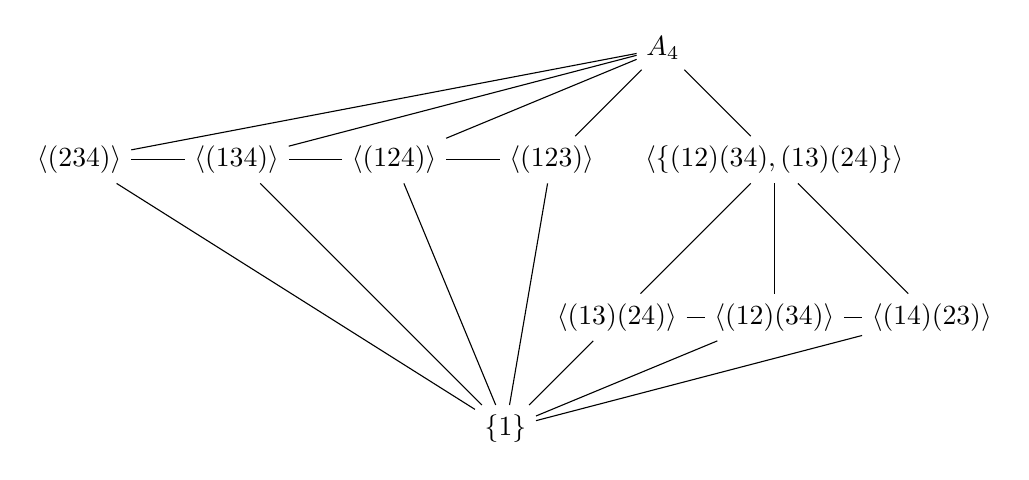
\begin{tikzpicture}[node distance=2cm]
\node(A4)                           {$A_4$};
\node(V4)       [below right of=A4] {$\langle \{(12)(34), (13)(24)\}\rangle$};
\node(C31)      [below left of=A4]  {$\langle (123) \rangle$};
\node(C32)      [left of=C31]       {$\langle (124) \rangle$};
\node(C33)      [left of=C32]       {$\langle (134) \rangle$};
\node(C34)      [left of=C33]       {$\langle (234) \rangle$};
\node(C22)      [below of=V4]       {$\langle (12)(34)\rangle$};
\node(C21)      [left of=C22]       {$\langle (13)(24)\rangle$};
\node(C23)      [right of=C22]      {$\langle (14)(23)\rangle$};

\node(1)            [below left of=C21]     {$\left\{1\right\}$};
\draw(A4)       -- (V4);
\draw(A4)       -- (C31);
\draw(A4)       -- (C32);
\draw(A4)       -- (C33);
\draw(A4)       -- (C34);
\draw(C31)      -- (C32);
\draw(C32)      --  (C33);
\draw(C33)      --  (C34);
\draw(C31)      --  (1);
\draw(C32)      --  (1);
\draw(C33)      --  (1);
\draw(C34)      --  (1);
\draw(V4)       -- (C21);
\draw(V4)       -- (C22);
\draw(V4)       -- (C23);
\draw(C21)      -- (C22);
\draw(C22)      -- (C23);
\draw(C21)      --  (1);
\draw(C22)      --  (1);
\draw(C23)      --  (1);
\end{tikzpicture}
\end{center}
Weiter geht es mit den Konjugationsklassen. Ganz allgemein gilt für $\sigma \in \Sf_n$ und $(a_1 a_2 \cdots a_k) \in \Sf_n$:
\begin{equation}
\sigma \circ (a_1a_2 \cdots a_k) \circ \sigma^{-1} = \left(\sigma (a_1) \sigma (a_2) \cdots \sigma (a_k) \right) \, (\ast),
\end{equation}
also z.B. 
\begin{equation}
(124) \circ (123) \circ (124)^{-1} = (124) \circ (123)\circ (142) = (1)(234) = (234).
\end{equation}
Dies hilft, die Konjugationsklassen zu bestimmen. Diese sind:
\begin{align}
[(1)]&=\{(1)\} = Z(G)\\
[(12)(34)]&=\{(12)(34), (13)(24),(14)(23)\}\\
[(123)]&=\{(123), (142), (134), (243)\}\\
[(132)] &= \{(132), (124), (143), (234)\}
\end{align}
Die Überlegung, dass die unteren beiden Konjugationsklassen nicht eine gemeinsame Konjugationsklasse bilden, folgt daraus, dass die Kardinalität der entstehenden Untergruppe $8$ wäre, und $8$ nicht $12$ teilt. Damit haben wir die Klassengleichung bestimmt:
\begin{equation}
12 = 1+3+4+4
\end{equation}
Daraus können wir direkt ablesen, dass es keine Untergruppen der Ordnung $6$ geben kann. Gäbe es nämlich eine solche Untergruppe $A \leq A_4$, hätte diese Index $2$, und jede Gruppe von Index $2$ ist normal. Damit wäre $A$ normal, also eine Vereinigung von Konjugationsklassen von $A_4$. Dann müsste die Summe von Summanden der Klassengleichung $6$ ergeben, das ist aber unmöglich.
\end{beispiel}
\begin{übung}
Verifiziere $(\ast)$. Beweise, dass Untergruppen mit Index $2$ normal sind. Zeige, dass normale Untergruppen als Vereinigung von Konjugationsklassen geschrieben werden können.
\end{übung}
\begin{definition}{Zykeltyp}{zykeltyp}
Sei $\Sf_n$ die symmetrische Gruppe. Ein $\sigma \in \Sf_n$ kann als Produkt
\begin{equation}
\sigma = \sigma_1 \circ \sigma_2 \circ \cdots \sigma_k
\end{equation}
paarweise disjunkter Zykel $\sigma_i$ der Länge $m_i \geq 2$ geschrieben werden, wobei $(1)=\sigma_0$ gilt. O.B.d.A sei $m_1 \geq m_2 \geq \cdots \geq m_k$. Dann heißt der $k$-Tupel 
\begin{equation}
(m_1, m_2, \cdots, m_k)
\end{equation}
\textbf{Zykeltyp} von $\sigma$.
\end{definition}
\begin{satz}{Zykeltyp bestimmt Konjugationsklasse}{zykelkonjugation}
Zwei Elemente $\sigma, \sigma' \in \Sf_n$ sind genau dann in der gleichen Konjugationsklasse, wenn sie den gleichen Zykeltyp haben.
\end{satz}
\begin{beweis}
Übung 3.2
\end{beweis}
\subsection{Euklidische Bewegungen}
\label{subsec:euklidbewegungen}
Wir beginnen mit einer Widerholdung von Grundbegriffen:
\begin{definition}{Skalarprodukt, Norm, Metrik}{skalarprodukt}
Sei $v = (v_1 \cdots v_n)^T, w = (w_1 \cdots w_n)^T \in \R^n$ mit $n \geq 1$. Wir definieren das \textbf{Skalarprodukt} von $v$ mit $w$ als
\begin{equation}
\langle v,w \rangle := \Sum{i,1,n} v_iw_i \in \R
\end{equation}
und die \textbf{euklidische Norm}
\begin{equation}
\|v\| := \sqrt{\langle v, v \rangle} \in \R_{\geq 0}.
\end{equation}
Dies induziert den \textbf{euklidischen Abstand}
\begin{equation}
d(v,w) := \|v-w\|
\end{equation}
auf $\R^n$.
\end{definition}
Daraus erhalten wir einen speziellen Isometriebegriff für den $\R^n$:
\begin{definition}{Euklidische Bewegung}{euklidbeweg}
Eine Abbildung 
\begin{equation}
T: \R^n \to \R^n
\end{equation}
heißt \textbf{(euklidische) Bewegung} oder \textbf{(euklidische) Isometrie}, falls für alle $v,w \in \R^n$ gilt:
\begin{equation}
d(Tv,Tw) = d(v,w).
\end{equation}
Die Menge $E(n)$ der euklidischen Bewegungen mit der Komposition als Verknüpfung bildet eine Gruppe.
\end{definition}
\begin{bemerkung}
Die Injektivität von $T \in E(n)$ ist klar, die Injektivität folgt aus untenstehendem Korollar \ref{allgisoform}.
\end{bemerkung}
\begin{beispiele} Wir schauen uns Beispiele für euklidische Isometrien an:
\begin{enumerate}
\item Für jedes $b \in \R^n$ sind die \textbf{Translationen}
\begin{equation}
\begin{split}
\tau_b: \R^n &\to \R^n \\
v &\mapsto v + b
\end{split}
\end{equation}
Isometrien.
\item Für jede Matrix $A \in \text{O}(n,\R)$ ist die Abbildung
\begin{equation}
\begin{split}
\mu_A: \R^n &\to \R^n\\
v &\mapsto Av
\end{split}
\end{equation}
eine Isometrie, denn es gilt $\langle v, w \rangle = v^Tw$, und damit
\begin{equation}
\langle Av, Aw \rangle = (Av)^T Aw = v^T A^T A w = v^T w = \langle v, w \rangle.
\end{equation}
Für den Abstand gilt dann:
\begin{equation}
d(Av,Aw) = \| Av-Aw\| = \|A(v-w)\| = \sqrt{\langle A(v-w), A(v-w) \rangle} = \|v-w\| = d(v,w),
\end{equation}
also ist $\mu_A$ tatsächlich eine euklidische Isometrie.
\end{enumerate}
\end{beispiele}
\begin{satz}{Euklidische Bewegungen sind orthogonale Transformationen}{eulidistortho}
Sei $T \in E(n)$ mit $T(0) = 0$. Dann existiert ein $A \in \text{O}(n, \R)$, sodass $T = \mu_A$.
\end{satz}
\begin{beweis}
\begin{enumerate}
\item Zuerst zeigen wir, dass $T$ das Skalarprodukt erhält:
\begin{equation}
T \in E(n) \implies \langle Tv-Tw, Tv-Tw\rangle = d(Tv,Tw)^2 = \langle v-w, v-w \rangle \, (\ast).
\end{equation}
Setze $w = 0$. Dann gilt 
\begin{equation}
 \langle Tv, Tv \rangle = Tv-T0 = \langle v-0, v-0 \rangle = \langle v,v \rangle
\end{equation}
Mit der Bilinearität des Skalarprodukts erhalten wir
\begin{equation}
\langle Tv,Tv \rangle - \langle Tv,Tw \rangle - \langle Tw, Tv \rangle + \langle Tw, Tw \rangle =^{(\ast)} \ip{v,v} - \ip{v,w} - \ip{w,v} + \ip{w,w}.
\end{equation}
Da das Skalarprodukt darüber hinaus symmetrisch ist, folgt
\begin{equation}
-2 \ip{Tv,Tw} = -2 \ip{v,w}.
\end{equation}
\item Falls zusätzlich für alle $1 \leq i \leq n$ gilt, dass $Te_i = e_i$, so ist $T = \id$. Für $v \in \R^n$ gilt dann:
\begin{equation}
(Tv)_i = \langle Tv, e_i \rangle =  \langle Tv, Te_i \rangle = \langle v, e_i \rangle = v_i.
\end{equation}
\item Sei nun $T$ wieder allgemein mit $T(0)=0$. Setze
\begin{equation}
A:=(Te_1 Te_2 \cdots Te_n) \in \R^{n \times n}
\end{equation}
mit Spaltenvektoren $Te_i$. Wegen $\langle Te_i, Te_j \rangle =^1 \langle e_i , e_j \rangle$ gilt $A \in \text{O}(n,\R)$. Zudem ist $\mu_{A^\text{T}} \circ T =: \widetilde{T} \in E(n)$ mit $\widetilde{T}(0) = 0$ für alle $i$. Also $\widetilde{T}e_i = e_i$ und damit $\widetilde{T} = \id$.
\end{enumerate}
\end{beweis}
\begin{korollar}{aus Satz \ref{eulidistortho}}{allgisoform}
Jede Isometrie $T \in E(n)$ ist von der Form
\begin{equation}
\begin{split}
T: \R^n &\to \R^n\\
v &\mapsto Av + b
\end{split}
\end{equation}
für $A \in \text{O}(n,\R)$ und $b \in \R^n$.
\end{korollar}
\begin{beweis}
Sei $b:=T(0)$. Dann gilt
\begin{equation}
\tau_{-b}\circ T(0) = 0.
\end{equation}
Nach Satz \ref{eulidistortho} gilt $\tau_{-b} \circ T = \mu_A$ für $A \in \text{O}(n,\R)$. Also ist $T = \tau_b \circ \mu_A$.
\end{beweis}
\begin{definition}{Direktes Produkt}{direktesprod}
Seien $G$ und $G'$ Gruppen. Dann heißt die Gruppe $G \times G'$ mit der Verknüpfung
\begin{equation}
\begin{split}
(G \times G') \times (G \times G') &\to G \times G'\\
((g,h), (g',h')) &\mapsto (g\circ g', h \circ h')
\end{split}
\end{equation}
\textbf{direktes Produkt} von $G$ und $G'$.
\end{definition}
\begin{bemerkung}
Es existiert also eine Bijektion
\begin{equation}
E(n) \cong \{(A,b) \, | \, A \in \text{O}(n, \R), b \in \R^n\},
\end{equation}
wobei das Kompositionsgesetz durch
\begin{equation}
(A,b) \circ (A', b') = (AA', Ab'+b)
\end{equation}
gegeben ist. Also ist $E(n) = O(n, \R) \times \R^n$ als Menge, aber nicht als Gruppe!
\end{bemerkung}
\begin{definition}{Semidirektes Produkt}{semidirektesprodukt}
Seien $H$ und $N$ Gruppen und wirke $H$ auf $N$ via Gruppenhomomorphismen, also:
\begin{enumerate}
\item $H \acts G$.
\item Für jedes $h \in H$ ist die Abbildung $N \to N, \, x \mapsto h.x$ ein Gruppenhomomorphismus.
\end{enumerate}
Dann definieren wir eine Verknüpfung auf $H \times N$ durch:
\begin{equation}
\begin{split}
\circ: (H \times N) \times (H \times N) &\to H \times N\\
\left( (h,x) , (h', x')\right) &\mapsto \left( (hh', x(hx') \right).
\end{split}
\end{equation}
Dies definiert eine Gruppenstruktur auf $H \times N$, genannt \textbf{semidirektes Produkt} $H \ltimes N$ von $(H,N, H\acts N)$.
\end{definition}
\begin{übung}
Man zeige, dass $H \ltimes N$ tatsächlich eine Gruppe ist.
\end{übung}
\begin{beispiele}
\begin{enumerate}
\item Falls $H \acts N$ die triviale Wirkung ist, so ist $H \ltimes N = H \times N$.
\item Betrachte die Wirkung $\text{O}(n,\R) \acts \R^n$ durch Matrixmultiplikation. Dann gilt $E(n) \cong \text{O}(n,\R) \ltimes \R^n$ als Gruppen.
\item Sei $T \in E(2)$ mit $T(0) = 0$. Dann gilt $T = \mu_A$ mit $A \in \text{O}(n, \R)$. Falls $T$ orientierungserhaltend ist, gilt sogar $A \in \text{SO}(2, \R)$, also 
\begin{equation}
A = \mat{\cos \theta, - \sin \theta}{\sin \theta, \cos \theta}
\end{equation}
für $\theta \in \quotient{\R}{2\pi \Z}$. Also sind die Isometrien der Form $\mu_A, A \in \text{SO}(2,\R)$ genau die Drehungen um den Ursprung. Alle Bewegungen $T \in E(2)$ sind Kompositionen von Translationen, Spiegelungen und Drehungen.
\end{enumerate}
\end{beispiele}
\begin{definition}{Kurze exakte Sequenz}{kes}
Eine \textbf{kurze exakte Sequenz} von Gruppen ist gegeben durch 
\begin{center}
\begin{tikzcd}
    \{1\} \arrow[r] & N \arrow[r, "i"] & G \arrow[r, "p"] &H \arrow[r] &\{1\}, 
\end{tikzcd}
\end{center}
wobei:
\begin{itemize}
\item $N,G$ und $H$ Gruppen sind.
\item $i: N \to G$ ein injektiver Gruppenhomomorphismus (Monomorphismus) ist.
\item $p: G \to H$ ein surjektiver Gruppenhomomorphismus (Epimorphismus) ist.
\item $\im (i) = \ker (p)$ gilt.
\end{itemize}
Eine kurze exakte Sequenz \textbf{zerfällt}, falls ein Homomorphismus $s: H \to G$ mit $p \circ s = \id_H$ existiert.
\end{definition}
\begin{satz}{Kurze exakte Sequenzen und semidirekte Produkte}{kessemidirekt}
\begin{enumerate}
\item Seien $H,N$ Gruppen und $H$ wirke auf $N$ via Homomorphismen. Dann existiert eine zerfallende kurze exakte Sequenz:
\begin{center}
\begin{tikzcd}
    \{1\} \arrow[r] & N \arrow[r, "i"] & N \rtimes H \arrow[r, "p"] &H \arrow[r] &\{1\}. 
\end{tikzcd}
\end{center}
\item Sei 
\begin{center}
\begin{tikzcd}
    \{1\} \arrow[r] & N \arrow[r, "i"] & G \arrow[r, "p"] &H \arrow[r] &\{1\}. 
\end{tikzcd}
\end{center}
eine zerfallende kurze exakte Sequenz mit Schnitt $s$. Dann definiert Konjugation mit $s(H)$ eine Wirkung von $H$ auf $N$ via Homomorphismen, sodass $G \cong N \rtimes H$ ist:
\begin{center}
\begin{tikzcd}
    \{1\} \arrow[r] & N \arrow[r, "i"] & G \arrow[r, "p"] \arrow[d, "\phi"] &H \arrow[r] &\{1\}\\
    \{1\} \arrow[r] & N \arrow[r, "i"] & N \rtimes H \arrow[r, "p"] &H \arrow[r] &\{1\}.
\end{tikzcd}
\end{center}
\end{enumerate}
\end{satz}
\begin{beweis}
Übung 4.4
\end{beweis}
Wir versuchen jetzt, die $\text{O}(3,\R) \supseteq \text{SO}(3, \R)$ zu verstehen.
\begin{definition}{Drehung}{drehung}
Eine \textbf{Drehung von} $\R^3$ um den Ursprung $0 \in \R^3$ ist eine Drehung um einen Winkel $\theta \in \quotient{R}{2 \pi \Z}$ um eine Achse aufgespannt von $v \in \R^3 \exc \{0\}$.
\end{definition}
\begin{satz}{Drehungen sind spezielle orthogonale Transformationen}{drehungistso}
Die Bewegungen der Form $\mu_A$ mit $A \in \text{SO}(3,\R)$ sind genau die Drehungen um $0$.
\end{satz}
\begin{beweis}
\begin{enumerate}
\item $A$ hat einen Eigenvektor $v \neq 0$ zum Eigenwert $1$, also $Av=v$. Dafür genügt es, $\det (A-I_3) = 0$ zu zeigen. Wir rechnen schrittweise:
\begin{enumerate}[(i)]
\item \begin{equation}
\det(A-I_3) = \det(A(I_3-A^\text{T})) = \det(A) \det(I_3 - A^\text{T}) = \det(I_3 - A^\text{T}) = \det(I_3 -A)
\end{equation}
\item \begin{equation}
\det(A-I_3) = \det(-(I-A)) = (-1)^3 \det(I_3-A)
\end{equation}
\end{enumerate}
Aus diesen beiden Gleichungen folgt bereits $\det(A-I_3) = 0$, was zu zeigen war.
\item Sei $v \neq 0$ ein Eigenvektor von $A$ zum Eigenwert $1$. O.B.d.A. sei $\|v\|=1$ (ersetze $v$ durch $\frac{v}{\|v\|}$). Ergänze $v$ mit Gram-Schmidt zu einer ONB $(v,p,q)$ des $\R^3$. Bezüglich dieser Basis hat $\mu_A$ die Form
\begin{equation}
\mat{1,0,0}{0,\ast,\ast}{0,\ast,\ast} \in \text{SO}(3,\R).
\end{equation}
Das sehen wir ein, da die erste Spalte der Abbildung des Eigenvektors $v$ entspricht. Nun ist die Abbildung orthogonal, also bleibt das Skalarprodukt erhalten. Damit muss im ersten Eintrag der zweiten und dritten Spalte $0$ sein, sonst wäre das Bild der ONB keine ONB. Die untere Blockdiagonalmatrix ist in $\text{SO}(2,\R)$, also gilt
\begin{equation}
\mat{\ast, \ast}{\ast, \ast} = \mat{\cos \theta, - \sin \theta}{\sin \theta, \cos \theta}.
\end{equation}
\end{enumerate}
Damit ist $\mu_A$ eine Drehung um die von $v$ aufgespannte Achse mit Winkel $\theta$.
\end{beweis}
\begin{korollar}{Aus Satz \ref{drehungistso}}{aussatzdrehungistso}
Die Menge der Drehungen von $\R^3$ um $0 \in \R^3$ bildet eine Gruppe unter Verknüpfung, die isomorph zu $\text{SO}(3,\R)$ ist.
\end{korollar}
\subsection{Symmetrie im Raum}
\label{subsec:symmetrieimraum}
\begin{definition}{Euklidische Symmetriegruppe}{euklidsymmetriegruppe}
Für eine Teilmenge $F \sub \R^3$, genannt \textbf{Figur}, definieren wir die \textbf{euklidische Symmetriegruppe}
\begin{equation}
\Sym (F) := \left\{ T \in E(3) | T(F) = F\right\} \leq E(3)
\end{equation}
und die \textbf{euklidische Drehsymmetriegruppe}
\begin{equation}
\Symso (F) := \left\{ A \in \text{SO}(3,\R) | \mu_A (F) = F\right\} \leq \text{SO}(3,\R)
\end{equation}
von $F$.
\end{definition}
\begin{satz}{Klassifikation der Drehgruppe in $\R^3$}{drehgruppenklass}
Jede endliche Untergruppe von $\text{SO}(3, \R)$ ist konjugiert zu einer der folgenden Gruppen:
\begin{enumerate}
\item $\left\{ \mat{1,0,0}{0,1,0}{0,0,1} \right\}$: triviale Gruppe
\item Die zyklische Gruppe $\text{C}_n$ der Ordnung $n$, gegeben durch die Drehgruppe $\Symso (P)$ einer Pyramide $P$ über einem regulären $n$-Eck mit Mittelpunkt $0$.
\item Die Drehgruppe $\text{D}_n$ der Ordnung $2n$, gegeben durch die Drehgruppe eines regulären Prismas über einem regulären $n$-Eck mit $n\geq 2$ und Mittelpunkt $0$.
\item Die Gruppe $A_4$, gegeben als Drehgruppe eines Tetraeders.
\item Die Gruppe $\Sf_4$, gegeben als Drehgruppe eines Würfels oder eines Oktaeders.
\item Die Gruppe $A_5$, gegeben als Drehgruppe eines Dodekaeders oder Ikosaeders.
\end{enumerate}
\end{satz}
\begin{figure}[H]
\centering
\begin{tikzpicture}
\coordinate (d1) at (0,2,0);
\node (d2) at (0,-1,0) {$\text{C}_6$};
\draw[red] (d1) -- (d2);
\begin{scope}[canvas is xz plane at y=0]
\coordinate (a) at (xyz spherical cs: radius=1, longitude=0);
\coordinate (b) at (xyz spherical cs: radius=1, longitude=60);
\coordinate (c) at (xyz spherical cs: radius=1, longitude=120);
\coordinate (d) at (xyz spherical cs: radius=1, longitude=180);
\coordinate (e) at (xyz spherical cs: radius=1, longitude=240);
\coordinate (f) at (xyz spherical cs: radius=1, longitude=300);
\draw  (a) -- (b) -- (c) -- (d) -- (e) -- (f) -- (a);
\end{scope}
\begin{scope}[canvas is xz plane at y=1.5]
\coordinate (s) at (xyz spherical cs: radius=0);
\end{scope}
\draw (a) -- (s);
\draw (b) -- (s);
\draw (c) -- (s);
\draw (d) -- (s);
\draw (e) -- (s);
\draw (f) -- (s);
\coordinate (t) at (1.5,0,1.5);
\coordinate (u) at (-1.5,0,1.5);
\coordinate (v) at (-1.5,0,-1.5);
\coordinate (w) at (1.5,0,-1.5);
\draw (t) -- (u) -- (v) -- (w) -- (t);
\fill[nearly transparent, blue] (t) -- (u) -- (v) -- (w) -- (t);
\end{tikzpicture}
\begin{tikzpicture}
\coordinate (d1) at (0,2,0);
\node (d2) at(0,-2,0) {$\text{D}_6$};
\draw[red] (d1) -- (d2);
\begin{scope}[canvas is xz plane at y=1]
\coordinate (pa) at (xyz spherical cs: radius=1, longitude=0);
\coordinate (pb) at (xyz spherical cs: radius=1, longitude=60);
\coordinate (pc) at (xyz spherical cs: radius=1, longitude=120);
\coordinate (pd) at (xyz spherical cs: radius=1, longitude=180);
\coordinate (pe) at (xyz spherical cs: radius=1, longitude=240);
\coordinate (pf) at (xyz spherical cs: radius=1, longitude=300);
\draw  (pa) -- (pb) -- (pc) -- (pd) -- (pe) -- (pf) -- (pa);
\end{scope}
\begin{scope}[canvas is xz plane at y=0]
\coordinate (a) at (xyz spherical cs: radius=1, longitude=0);
\coordinate (b) at (xyz spherical cs: radius=1, longitude=60);
\coordinate (c) at (xyz spherical cs: radius=1, longitude=120);
\coordinate (d) at (xyz spherical cs: radius=1, longitude=180);
\coordinate (e) at (xyz spherical cs: radius=1, longitude=240);
\coordinate (f) at (xyz spherical cs: radius=1, longitude=300);
\draw[dashed]  (a) -- (b) -- (c) -- (d) -- (e) -- (f) -- (a);
\end{scope}
\begin{scope}[canvas is xz plane at y=-1]
\coordinate (ma) at (xyz spherical cs: radius=1, longitude=0);
\coordinate (mb) at (xyz spherical cs: radius=1, longitude=60);
\coordinate (mc) at (xyz spherical cs: radius=1, longitude=120);
\coordinate (md) at (xyz spherical cs: radius=1, longitude=180);
\coordinate (me) at (xyz spherical cs: radius=1, longitude=240);
\coordinate (mf) at (xyz spherical cs: radius=1, longitude=300);
\draw  (ma) -- (mb) -- (mc) -- (md) -- (me) -- (mf) -- (ma);
\end{scope}
\draw (pa) -- (ma);
\draw (pb) -- (mb);
\draw (pc) -- (mc);
\draw (pd) -- (md);
\draw (pe) -- (me);
\draw (pf) -- (mf);
\coordinate (t) at (1.5,0,1.5);
\coordinate (u) at (-1.5,0,1.5);
\coordinate (v) at (-1.5,0,-1.5);
\coordinate (w) at (1.5,0,-1.5);
\draw (t) -- (u) -- (v) -- (w) -- (t);
\fill[nearly transparent, blue] (t) -- (u) -- (v) -- (w) -- (t);
\end{tikzpicture}
\begin{tikzpicture}
\coordinate (d1) at (0,2,0);
\node (d2) at (0,-1,0) {$\text{A}_4$};
\draw[red] (d1) -- (d2);
\begin{scope}[canvas is xz plane at y=0]
\coordinate (a) at (xyz spherical cs: radius=1, longitude=0);
\coordinate (b) at (xyz spherical cs: radius=1, longitude=120);
\coordinate (c) at (xyz spherical cs: radius=1, longitude=240);
\draw  (a) -- (b) -- (c) -- (a);
\end{scope}
\begin{scope}[canvas is xz plane at y=1.5]
\coordinate (s) at (xyz spherical cs: radius=0);
\end{scope}
\draw (a) -- (s);
\draw (b) -- (s);
\draw (c) -- (s);
\coordinate (t) at (1.5,0,1.5);
\coordinate (u) at (-1.5,0,1.5);
\coordinate (v) at (-1.5,0,-1.5);
\coordinate (w) at (1.5,0,-1.5);
\draw (t) -- (u) -- (v) -- (w) -- (t);
\fill[nearly transparent, blue] (t) -- (u) -- (v) -- (w) -- (t);
\end{tikzpicture}
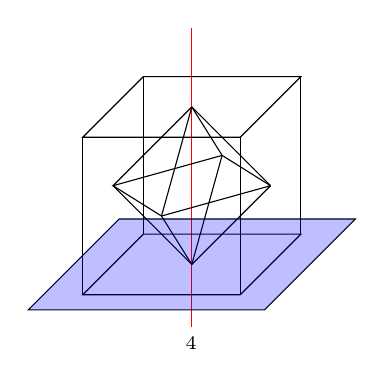
\begin{tikzpicture}
\coordinate (d1) at (0,3,0);
\node (d2) at(0,-1,0) {$\Sf_4$};
\draw[red] (d1) -- (d2);
\coordinate (os1) at (0,2,0);
\coordinate (os2) at (0,0,0);
\coordinate (oa) at (1,1,0);
\coordinate (ob) at (0,1,-1);
\coordinate (oc) at (-1,1,0);
\coordinate (od) at (0,1,1);
\draw (oa) -- (ob) -- (oc) -- (od) -- (oa);
\draw (oa) -- (os1);
\draw (oa) -- (os2);
\draw (ob) -- (os1);
\draw (ob) -- (os2);
\draw (oc) -- (os1);
\draw (oc) -- (os2);
\draw (od) -- (os1);
\draw (od) -- (os2);
\coordinate (pa) at (1,2,1);
\coordinate (pb) at (1,2,-1);
\coordinate (pc) at (-1,2,1);
\coordinate (pd) at (-1,2,-1);
\draw (pa) -- (pb) -- (pd) -- (pc) -- (pa);
\coordinate (a) at (1,0,1);
\coordinate (b) at (1,0,-1);
\coordinate (c) at (-1,0,1);
\coordinate (d) at (-1,0,-1);
\draw (a) -- (b) -- (d) -- (c) -- (a);
\draw (a) -- (pa);
\draw (b) -- (pb);
\draw (c) -- (pc);
\draw (d) -- (pd);
\coordinate (t) at (1.5,0,1.5);
\coordinate (u) at (-1.5,0,1.5);
\coordinate (v) at (-1.5,0,-1.5);
\coordinate (w) at (1.5,0,-1.5);
\draw (t) -- (u) -- (v) -- (w) -- (t);
\fill[nearly transparent, blue] (t) -- (u) -- (v) -- (w) -- (t);
\end{tikzpicture}
\begin{tikzpicture}
\coordinate (d1) at (0,2,0);
\node (d2) at(0,-2,0) {$A_5$};
\draw[red] (d1) -- (d2);
\begin{scope}[canvas is xz plane at y=0.5]
\coordinate (pa) at (xyz spherical cs: radius=1, longitude=0);
\coordinate (pb) at (xyz spherical cs: radius=1, longitude=360/5);
\coordinate (pc) at (xyz spherical cs: radius=1, longitude=360/5*2);
\coordinate (pd) at (xyz spherical cs: radius=1, longitude=360/5*3);
\coordinate (pe) at (xyz spherical cs: radius=1, longitude=360/5*4);
\draw  (pa) -- (pb) -- (pc) -- (pd) -- (pe) -- (pa);
\end{scope}
\begin{scope}[canvas is xz plane at y=-0.5]
\coordinate (ma) at (xyz spherical cs: radius=1, longitude=36);
\coordinate (mb) at (xyz spherical cs: radius=1, longitude=36+72);
\coordinate (mc) at (xyz spherical cs: radius=1, longitude=36+72*2);
\coordinate (md) at (xyz spherical cs: radius=1, longitude=36+72*3);
\coordinate (me) at (xyz spherical cs: radius=1, longitude=36+72*4);
\draw  (ma) -- (mb) -- (mc) -- (md) -- (me) -- (ma);
\end{scope}
\begin{scope}[canvas is xz plane at y=-1]
\coordinate (ms) at (xyz spherical cs: radius=0);
\draw  (ma) -- (ms);
\draw  (mb) -- (ms);
\draw  (mc) -- (ms);
\draw  (md) -- (ms);
\draw  (me) -- (ms);
\end{scope}
\begin{scope}[canvas is xz plane at y=1]
\coordinate (ps) at (xyz spherical cs: radius=0);
\draw  (pa) -- (ps);
\draw  (pb) -- (ps);
\draw  (pc) -- (ps);
\draw  (pd) -- (ps);
\draw  (pe) -- (ps);
\end{scope}
\draw (pa) -- (ma);
\draw (pa) -- (me);
\draw (pb) -- (mb);
\draw (pb) -- (ma);
\draw (pc) -- (mc);
\draw (pc) -- (mb);
\draw (pd) -- (md);
\draw (pd) -- (mc);
\draw (pe) -- (me);
\draw (pe) -- (md);
\coordinate (t) at (1.5,0,1.5);
\coordinate (u) at (-1.5,0,1.5);
\coordinate (v) at (-1.5,0,-1.5);
\coordinate (w) at (1.5,0,-1.5);
\draw (t) -- (u) -- (v) -- (w) -- (t);
\fill[nearly transparent, blue] (t) -- (u) -- (v) -- (w) -- (t);
\end{tikzpicture}
\caption{Klassifikation der Drehgruppe $\text{SO}(3,\R)$.}
\end{figure}

\begin{beweis}
O.B.d.A. sei $G \leq \text{SO}(3,\R)$ eine endliche Untergruppe mit $G \neq \{I_3\}$. In Abschnitt \ref{subsec:euklidbewegungen} haben wir gezeigt, dass jedes $A \in \text{SO}(3,\R)$, $A \neq I_3$ eine Drehung um eine Achse $l = \langle v \rangle \sub \R^3$. Wir bezeichnen die zwei Elemente der Menge $l \cap \S^2$ mit $\S^2 := \{ v \in \R^3| \|v\| = 1\}$ als \textbf{Pole von} $A$. Wir bezeichnen weiterhin mit $P \sub \S^2$ die Menge aller Pole aller Elemente $A \in G$, $A \neq I_3$.
\begin{enumerate}
\item Die Operation $G \acts \R^3$ via Links-Matrixmultiplikation schränkt sich ein auf eine Operation $G \acts P$. Sei dazu $P$ ein Pol von $A \in G$, $A \neq I_3$ und sei $B \in G$. Dann gilt
\begin{equation}
(BAB^{-1})B.p = B(AB^{-1}B).p = BA.p = B.p,
\end{equation}
da Pole von $A$ invariant unter $A$ sind. Also ist $B.p$ ein Pol von $A' = B AB^{-1} \in G$.
\end{enumerate}
\end{beweis}
\begin{lemma}{Klassifikation von $\text{SO}(2,\R)$}{so2klass}
Sei $0 \neq p \in \R^3$ und $H \leq \Symso (\R^3)_p$ eine endliche Untergruppe von Drehungen um die Achse $0_p \in \R^3$.\footnote{Notationell ist $\Symso (\R^3)_p$ der Stabilisator von $p$ unter $\Symso (\R^3) \acts \R^3$.} Dann ist $H$ zyklisch, erzeugt von der Drehung $\delta_\theta$ in $H$ um den kleinsten Winkel $0<\theta \leq 2\pi$ gegen den Uhrzeigersinn.
\end{lemma}
\begin{beweis}
Sei $\delta_\theta \in H$ eine Drehung um den kleinsten Winkel. Diese existiert, da 
\begin{equation}
\{\theta \in (0,2\pi)|\delta_\theta \in H\} \sub \R
\end{equation}
eine endliche, nicht-leere Teilmenge ist. Wir behaupten, dass $H = \langle \delta_\theta \rangle$. Wäre dem nicht so, gäbe es $\phi \in (0,2\pi)$ und $n \in \N$, sodass $n\theta < \phi < (n+1) \theta$ mit $\delta_\phi \in H$. Dann gilt aber 
\begin{equation}
\delta_{\phi - n\theta} = \delta_\phi (\delta_\theta^n)^{-1} \in H
\end{equation}
mit $0 < \phi - n\theta < \theta$, was ein Widerspruch zur Annahme ist.
\end{beweis}
\begin{beweis}
Wir machen weiter im Beweis von Satz \ref{drehgruppenklass}. 
\begin{enumerate}
\setcounter{enumi}{1}
\item Für $p \in P$ besteht $G_p \leq G$ genau aus den Drehungen $\delta_\theta$ mit $\theta \in \quotient{\R}{2\pi \Z}$ um die Achsen $O_p$ mit $\delta_\theta \in G$. Gemäß Lemma \ref{so2klass} gilt also $G_p = \langle \delta_\theta \rangle$, wobei $\delta_\theta$ der kleinste Winkel mit $\delta_\theta \in G_p$ ist. Da $p \in P$ ein Pol ist, ist $G_p \neq \langle I_3 \rangle$. Es gilt $\theta = \frac{2\pi}{r_p}$ mit $r_p = |G_p|$ und $r_p > 1$, da $p$ ein Pol ist. Wir definieren $n_p := |G.p|$ und betrachten die Bahnformel
\begin{equation}
N:=|G| = n_p \cdot r_p.
\end{equation}
\item Betrachte die Menge
\begin{equation}
X := \{(p,A)\,|\, p \in P \, \text{ist Pol von} \, A \in G\} \sub P \times G.
\end{equation}
Da jedes $I_3 \neq A \in G$ genau zwei Pole hat, gilt $|X| = 2N-2$. Fixieren wir andererseits einen Pol $p$, dann hat die Menge $\{I_3 \neq A \in G \, | \, p \, \text{Pol von} \, A \} = G_p \exc \{I_3\}$ die Kardinalität $r_p-1$. Also gilt $|X| = \sum_{p \in P} (r_p -1) = 2N-2$. Für $p' \in G.p$ gilt: $|G_p| = |G_{p'}|$, also $r_p = r_{p'}$. Wir erhalten insgesamt:
\begin{equation}
\sum_{G.p \in \invquotient{G}{P}} n_p(r_p-1) = 2N-2.
\end{equation}
Division beider Seiten durch $N = n_pr_p$ liefert
\begin{equation}
\label{eq:drehgruppenbahngl}
\sum_{G.p \in \invquotient{G}{P}} \left(1- \frac{1}{r_p}\right) = 2-\frac{2}{N}.
\end{equation}
\item Aus Gleichung \ref{eq:drehgruppenbahngl} folgt sofort, dass höchstens drei Bahnen existieren können, also $\left|\invquotient{G}{P}\right| \leq 3$.
\begin{enumerate}[1. {Fall}:]
\item Sei $\left|\invquotient{G}{P}\right| =1$. Dann gilt gemäß Gleichung \ref{eq:drehgruppenbahngl}: 
\begin{equation}
\underbrace{-\frac{1}{r}}_{<1} = \underbrace{-\frac{2}{N}}_{\geq 1}
\end{equation}
für $r = |G_p|$, $p \in P$, was ein Widerspruch ist. Solche Bahnen existieren somit nicht.
\item Sei $\left|\invquotient{G}{P}\right| =2$, also 
\begin{align}
\left( 1 - \frac{1}{r_1}\right) + \left(1 - \frac{1}{r_2} \right) &= 2 - \frac{2}{N}\\
\iff \frac{2}{N} &= \frac{1}{r_1}+ \frac{1}{r_2}.
\end{align}
Es gilt aber $r_i \leq N$, also $r_1=r_2=N$ und damit $n_1=n_2=1$. Es gibt somit zwei Pole $P=\{\pm p\}$, die von allen Gruppenelementen stabilisiert werden. Also ist $G \leq \Symso (\R^3)_p$ eine endliche Gruppe von Drehungen um die Achse $0_p$ (sowie um die Achse $\overline{(-p)p}$). Mit Lemma \ref{so2klass} folgt
\begin{equation}
G = \langle \delta_\theta \rangle \sim \text{C}_n.
\end{equation}
\item Sei $\left|\invquotient{G}{P}\right| =3$, also 
\begin{equation}
\frac{2}{N} = \frac{1}{r_1} + \frac{1}{r_2} + \frac{1}{r_3} - 1.
\end{equation}
O.B.d.A. sei $r_1 \leq r_2 \leq r_3$. Falls alle $r_i \geq 3$ sind, ist dies ein Widerspruch, also $r_1 = 2$. Wir unterscheiden weitere Fälle:
\begin{enumerate}[{3.}1. {Fall:}]
\item Sei $r_2=2$, dann ist $r_3 = \frac{N}{2}$ und $N=2r_3$ gerade.
\item Sei $r_2=3$ und $r_3 = 3$. Dann ist $N = (2, n_i = (6,4,4))$.
\item Sei $r_2 = 3$ und $r_3 = 4$, dann ist $N=24$ und $n_i = (12,8,6)$.
\item Sei $r_2=3$ und $r_3 =5$, dann ist $N=60$ und $n_i=(30,20,12)$.
\end{enumerate}
\end{enumerate}
\item Jetzt müssen wir noch die verschiedenen Fälle aus dem 4. Schritt genauer untersuchen.
\begin{enumerate}[(I)]
\item Es existieren zwei Bahnen, bestehend aus je einem Pol, also $P=\{\pm p\}$. Daher ist $G=G_p$ eine endliche Gruppe von Drehungen um die von $p$ erzeugte Achse. Nach Lemma \ref{so2klass} ist die Gruppe zyklisch, erzeugt durch Drehungen um $\frac{2\pi}{N}$ durch $\overline{(-p)p}$. Sei $C \in \text{SO}(3,\R)$ eine Drehung, die die Standardkoordinate $e_3$ auf $p$ abbildet. Dann ist $C^{-1}GC: e_3 \to p \to p \to e_3$ genau die Drehgruppe $P_n$ der Pyramide.
\item 
\begin{enumerate}[(a)]
\item Für $n_3=2$ und $r_3=r$ hat die zugehörige Bahn zwei Pole $\{p,p'\}$. Für einen Pol $p$ existiert ein $I_3 \neq A$ mit $A_p = p$. Wegen $G \acts \{p,p'\}$ induziert $\{p,p'\} \to \{p,p'\}, x \mapsto Ax$ eine Selbstbijektion, also $Ap'=p'$ und damit $p'=-p$. Gemäß Lemma \ref{so2klass} ist der Stabilisator $G_p$ eine zyklische Gruppe der Ordnung $r$, erzeugt von einer Drehung $\delta$ um die Achse $\overline{0p}$ mit Winkel $\frac{2\pi}{r}$. Sei $tau \in \quotient{G}{G_p}$. Dann gilt $\tau.p = -p$, also ist $\tau$ eine Drehung um eine zu $p$ orthogonale Achse mit Winkel $\pi$. Damit erzeugt $\langle \delta, \tau \rangle \leq G$ eine Diedergruppe der Ordnung $2r$, also $G = \langle \delta, \tau \rangle$. Durch analogen Koordinatenwechsel mit $C \in \text{SO}(3,\R)$ wie in (I) gilt: $C^{-1}GC$ ist die Diedergruppe von $Z_r$.
\item Es gilt $n_3=4$ und $r_3=3$. Sei $B=\{p_1,p_2,p_3,p_4\}$ die zugehörige Bahn. Dann gilt $|G_{p_1}| = 3$ und $G_{p_1}$ besteht aus Drehungen um die von $p_1$ erzeugte Achse. Daher muss $G_p$ nicht trivial auf $\{p_2,p_3,p_4\}$ wirken, also nach der Bahnformel transitiv sein. Da $G_{p_1}$ durch Bewegungen wirkt, muss für die Skalarprodukte gelten:
\begin{equation}
\langle p_1,p_2 \rangle = \langle p_1, p_3 \rangle = \langle p_1, p_4 \rangle.
\end{equation}
Dieses Argument kann für jedes $i \in  \{1,2,3,4\}$ angewandt werden, wodurch wir Gleichheit von allen $\langle p_i, p_j \rangle$ für alle $1 \leq i \neq j \leq n$ erhalten. Weiterhin gilt $\langle p_i , p_j \rangle =1$ für alle $1 \leq i \leq n$. Mit der Bijektivität des Skalarprodukts folgt daraus, dass alle Abstände $\|p_i-p_j\|$ für $i \neq j$ gleich sind. Jeweils drei der vier Pole aus $B$ bilden also ein gleichseitiges Dreieck. Das impliziert, dass $B$ die Eckpunkte eines Tetraeders mit Schwerpunkt $0$ bildet.\\
Die Gruppe $G$ permutiert $B$ via Drehungen (lineare Abbildungen), also erhält $G$ $T'= \text{Konv}(B)$. Damit gilt $G \leq \text{SO}(T')$. Da $|G|=12$ und $|\text{SO}(T')|=12$ gilt, muss $G=\text{SO}(T')$ sein. Durch eine Drehung $C$ lässt sich $T$ überführen in eine Skalarstreckung von $T'$, also $C^{-1}GC=\text{SO}(T)$.
\item Es gilt $n_3 = 6$, $r_3 = 4$ und $N=24$. Sei $B:= \{p_1, \dots, p_6\}$ die zugehörige Bahn. Es gilt $|G_{p_1}|=4$, wobei $G_{p_1}$ die zyklische Gruppe von Drehungen um $p_i$ ist. Wegen der Bahnformel hat die Wirkung von $G_{p_1}$ auf $B\exc \{p_1\}$ einen Fixpunkt. Dann muss aber $p_2 = -p_1$ sein. Aus Lemma \ref{so2klass} folgt, dass $G_{p_1} =\langle \delta \rangle$ zyklisch der Ordnung $4$ ist. Die Bahnformel erlaubt zwei Möglichkeiten:
\begin{enumerate}[(i)]
\item $G_{p_1} \acts \{p_3, \dots, p_6\}$ zerfällt in zwei Bahnen der Kardinalität zwei. Seien diese Bahnen o.B.d.A. $\{p_3,p_4\}$ und $\{p_5,p_6\}$. Dann gilt aber $\delta.p_3 = p_4$ und $\delta.p_4 = p_3$. Das ist aber unmöglich, da $\delta$ eine Drehung um $90 \deg$ beschreibt.
\item $G_{p_1}$ wirkt transitiv, es gibt nur eine Bahn. Nach obigem Argument für $p_2 = -p_1$ muss o.B.d.A. gelten: $p_5 = -p_3$ und $p_6=-p_4$. Es folgt dann, dass $p_3,p_4,p_5$ und $p_6$ die Eckpunkte eines Quadrats in der Ebene senkrecht zu $p_1$ bilden.
\end{enumerate} 
\end{enumerate}
\end{enumerate}
\end{enumerate}
\textit{Der Rest verläuft analog und ist dem Leser überlassen.}
\end{beweis}
